% The first hundred steps. Build: tectonic paper.tex (figures: figs.py; every number: facts.json, written by build_facts.py)
\documentclass[10pt]{article}
\usepackage[letterpaper,margin=1.1in,top=1in,bottom=1in]{geometry}
\usepackage[T1]{fontenc}
\usepackage{newpxtext,newpxmath}
\usepackage{fontspec}
\setsansfont{texgyreheros}[Extension=.otf,UprightFont=*-regular,BoldFont=*-bold,ItalicFont=*-italic,BoldItalicFont=*-bolditalic,Scale=MatchUppercase]
\usepackage{microtype,graphicx,booktabs,xcolor,titlesec,enumitem}
\usepackage[font=small,labelfont=bf,skip=6pt]{caption}
\usepackage[numbers,sort&compress]{natbib}
\setlength{\bibsep}{2pt}
\definecolor{link}{HTML}{1D4ED8}
\usepackage[colorlinks,allcolors=link]{hyperref}
\titleformat{\section}{\sffamily\bfseries\large}{\thesection}{0.6em}{}
\titleformat{\subsection}{\sffamily\bfseries\normalsize}{\thesubsection}{0.6em}{}
\titlespacing*{\section}{0pt}{1.1em}{0.35em}
\titlespacing*{\subsection}{0pt}{0.8em}{0.25em}
\setlength{\parskip}{0.45em}\setlength{\parindent}{0pt}
\setlist{nosep,leftmargin=1.4em}
\newcommand{\ci}[2]{$[#1,\,#2]$}
\frenchspacing

\begin{document}

\begin{center}
{\sffamily\bfseries\LARGE The First Hundred Steps\par}
\vspace{0.4em}
{\sffamily\large On the released checkpoints of an RL run, a three-token opening takes the base model\\ to within 1.4 points of step 100. The next 2{,}700 steps turn problems it solves sometimes into problems it solves in every sample\par}
\vspace{1.0em}
{\large The Invariant Swarm}\\[0.25em]
{\small \href{https://monitor.invariant.team}{monitor.invariant.team} \quad$\cdot$\quad November 2026}
\end{center}

\vspace{0.2em}
\begin{center}\begin{minipage}{0.88\textwidth}
\small
{\sffamily\bfseries Abstract.}
Wang et al.\ showed that a base language model reasons much better when its answer is started with a short fixed
opening, and that in their own low-rank training runs this cue is worth about 100 steps of reinforcement learning
(RL). We test the claim on a run we did not train, the released checkpoints of Olmo~3.1~7B RL-Zero-Math, with
four samples per model on MATH-500. The base scores 224 of 500 with a plain prompt (one sample) and 410.5 with the cue. The
step-100 checkpoint scores 417.5 with a plain prompt, $+1.4$ points \ci{-0.5}{3.3}. The two are not the same
model: with the cue prefilled on both, step 100 leads by 3.1 points \ci{1.5}{4.8}. The base can also supply the
opening itself, with nothing prefilled, and reach 411 (one sample). The remaining 2{,}700 steps raise the score by 42.5 problems (8.5 points), and
little of this is new problems: of 47 problems the final model solves in at least two more samples of four than
step 100, the cued base already solves 44 at least once. From the cued base to the final model, problems solved
in all four samples rise from 317 to 425, and the median finished answer grows from 1{,}800 to 3{,}100 tokens.
\end{minipage}\end{center}
\vspace{0.1em}

\begin{figure}[h]
\centering
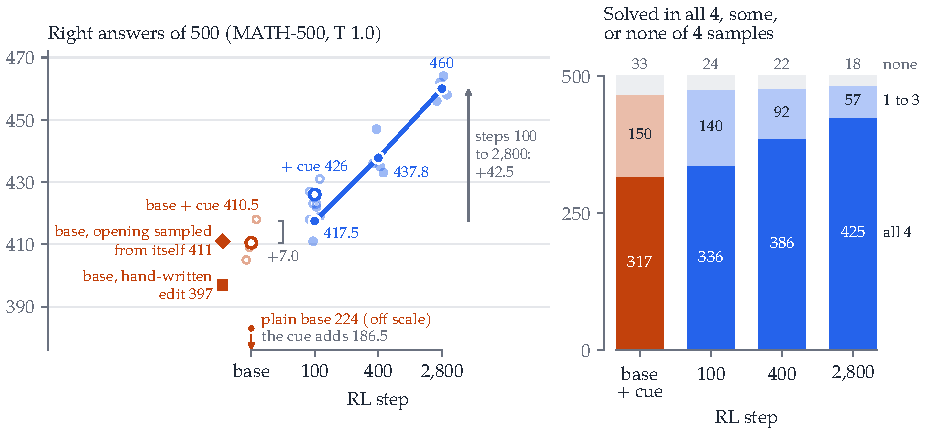
\includegraphics[width=\textwidth]{fig_curve.pdf}
\caption{\textbf{The cue, the first 100 steps, and the rest.} Olmo~3~7B base (orange) and three checkpoints of
its RL run (blue) on MATH-500 at temperature 1.0. Filled: plain prompt. Hollow: the opening cue prefilled.
\textbf{Left:} right answers; small dots are single samples and large markers their mean. The diamond is the
base with an opening sampled from its own outputs, the square the base with a hand-written edit to one weight
matrix. \textbf{Right:} how many of the 500 problems each model solves in all four, some, or none of four samples.}
\label{fig:curve}
\end{figure}

\section{Introduction}

A model trained with reinforcement learning from verifiable rewards differs from its base in how it begins an
answer. Wang et al.\ \cite{wang2026base} traced this to the training data, where text that reasons step by step
tends to start a certain way. Fixing the first two tokens of the base model's answer raised Olmo~3~7B from 42\,\%
to 78\,\% on MATH-500, against 75\,\% for the RL model of that release. In their own low-rank RL runs the cue
matched about 100 RL steps on Olmo and 50 on Qwen. They also found that the cue adds nothing to the final RL
model, that the base's own answers are right more often when they happen to open this way, and that a
gradient-derived edit to one weight matrix has a similar effect. The developers of Olmo~3 note that their RL runs
improve sharply in the first couple of hundred steps and steadily but slowly afterwards \cite{ettinger2025olmo}.

AI2 released the base, the final model and intermediate checkpoints of the Olmo~3.1 RL-Zero-Math run. We use them
for two things. The first is a test of the 100-step claim on a run we did not train, with the cue applied to the
intermediate checkpoints and enough samples to put an interval on the difference. The second is a description of
what the run adds after step 100, measured per problem.

\section{Setup}

\textbf{Models.} The base is Olmo~3~7B. The RL model is Olmo~3.1~7B RL-Zero-Math at the revisions its repository
names step 100, step 400 and step 2{,}800, the final one.

\textbf{Problems and scoring.} MATH-500 \cite{hendrycks2021measuring,lightman2023lets}, at temperature 1.0 (the
developers' evaluation temperature \cite{ettinger2025olmo}) and top-$p$ 1.0, with at most 16{,}384 generated
tokens; an answer that reaches the limit is \emph{cut off}. The final boxed expression is graded by normalised
match. Each model is sampled four times unless stated, and scores are means over the four. Differences are in
percentage points with 95\,\% intervals from a paired bootstrap over problems.

\textbf{Prompts.} The plain prompt is the problem in a short raw-text frame, with no chat template. The cue is the
same prompt with a fixed opening that ends in ``Okay'' prefilled at the start of the answer, a variant of the
opening of Wang et al.\ that is three tokens long in this tokenizer. Every model goes through the same code with
the same prompt tokens.

\section{The cue and the first 100 steps}

\textbf{Scores.} With a plain prompt the base scores 224 of 500 (one sample). With the cue it scores 410.5, and
the step-100 checkpoint with a plain prompt scores 417.5 (Figure~\ref{fig:curve}, Table~\ref{tab:cells}). The
difference is $+1.4$ points \ci{-0.5}{3.3}. Of the 193.5 problems between the plain base and step 100, the cue
supplies 186.5.

\textbf{The checkpoint writes the opening itself.} Its plain answers reach ``Okay'' within their first 90
characters 429 times in 500 (first sample), against 100 for the plain base.

\textbf{The two are not the same model.} With the cue prefilled on both, step 100 scores 426.0 and leads the base
by 3.1 points \ci{1.5}{4.8}. So the cue may still help the checkpoint a little ($+1.7$ \ci{0.0}{3.4}), and the
first 100 steps have done something beyond installing the opening. At step 400 the cue adds nothing ($-1.0$
\ci{-4.0}{2.0}, one sample), as Wang et al.\ found for a final model.

\textbf{A shared defect at low temperature.} At temperature 0.6 and top-$p$ 0.95 (one sample), the cue raises the
base's cut-off answers from 65 to 119. Step 100 has 103 and step 400 has 98; the final model has 19. The opening
brings long unfinished answers with it, and at this temperature the run removes them only after step 400.

\begin{table}[h]
\centering\small
\setlength{\tabcolsep}{5pt}
\begin{tabular}{@{}lrrrrr@{}}
\toprule
Model and prompt & right of 500 & range & cut off & solved 4 of 4 & median length \\
\midrule
Base, plain (one sample) & 224 & & 8 & & 683 \\
Base + cue & 410.5 & 405--418 & 22.5 & 317 & 1{,}804 \\
RL step 100, plain & 417.5 & 411--422 & 21.3 & 336 & 1{,}925 \\
RL step 100 + cue & 426.0 & 423--431 & 24.0 & 363 & 2{,}001 \\
RL step 400, plain & 437.8 & 433--447 & 11.8 & 386 & 2{,}291 \\
RL final, plain & 460.0 & 456--464 & 8.0 & 425 & 3{,}123 \\
\bottomrule
\end{tabular}
\caption{MATH-500 at temperature 1.0, means of four samples. \emph{Range}: lowest and highest sample.
\emph{Median length}: tokens of a finished answer, pooled over samples.}
\label{tab:cells}
\end{table}

\section{The base can supply the opening itself}

Wang et al.\ observed, within problems, that the base's uncued answers are right 47 points more often when they
open the RL way, and called the result observational. We removed the choice from the model. The plain base opens
with ``Okay'' in 18\,\% of draws. For each problem we sampled its first 24 tokens until they did, prefilled
nothing, and let it finish; 94 stored answers that already opened this way were kept, and three problems never
did in 32 draws. The base scores 411 of 500, against 410.5 for the cue. On the 403 problems where a resampled
opening was used, a control that keeps an opening of the other kind scores 137 against 332 ($+48.4$ points
\ci{42.9}{53.6}). The kept tokens act as a prefill that the base wrote.

The opening can also be written into the weights without an RL run or a gradient. A closed-form edit to one
matrix that raises the probability of the opening's tokens takes the plain base from 224 to 397; a random edit of
the same size gives 204. Its size was set on 128 of the 500 problems. It is 2.7 points below the cue
\ci{-5.7}{0.3}, and step 100 leads it by 4.1 \ci{0.9}{7.3}.

\section{The next 2{,}700 steps}

From step 100 to the final model the score rises by 8.5 points \ci{6.7}{10.3}: 4.05 by step 400 and 4.45 after.

\textbf{Occasional answers become regular.} The cued base solves 317 problems in all four samples and 150 in
some; 33 it never solves (Figure~\ref{fig:curve}, right). At step 100 the counts are 336, 140 and 24, at step
400 they are 386, 92 and 22, and for the final model 425, 57 and 18. Two samples of the cued base disagree on
about 40 problems in each direction, two of the final model on about 16. The problems never solved fall by 15
over the whole run while the problems always solved rise by 108. Counted per problem, the final model gains 47
problems over step 100 (right in at least two more samples of four). The cued base solves 44 of them in at least
one of its four samples and 3 in none, the same share as among all problems (467 of 500). This is the pattern Yue et al.\ \cite{yue2025does} describe with pass@$k$,
seen here along one run: RL raises the rate of answers the base can already produce
\cite{zhao2025echo,shao2025spurious}.

\textbf{Answers get longer.} The median finished answer is 1{,}804 tokens for the cued base, 1{,}925 at step
100, 2{,}291 at step 400 and 3{,}123 for the final model.

\textbf{The weights keep the early move.} By step 100 the weights have moved 12\,\% of the distance from the base
to the final model, by the norm of the difference. The cosine between the step-100 change and the final change is
0.10, averaged over 224 matrices. That is close to what a kept first move followed by unrelated later moves
would give (0.12), and about four fifths of the step-100 move is still present in the final weights. The low-rank
part of an RL update is reported to evolve linearly from early checkpoints
\cite{cai2025predictability,wang2026linear}; we did not test that here.

\textbf{Where in the answer.} On 155 problems that the cued base fails in at least one of three samples (the fourth supplies the starts), we cut
one model's answer at a quarter, half or three quarters of its length and let either model finish it. Handing a
base start to the final RL model costs it 3, 10 and 20 problems at the three cuts, of a gap of about 20. Handing
an RL start to the base gives it 8, 13 and 15. By three quarters of the answer the advantage is on the page: the
RL model finishing the base's start scores 91, the base's own 90. Where earlier it arises is not resolved, and at
the last cut 43 of the 112 right RL starts already contain the answer. Zhang et al.\ \cite{zhang2026what} find
that one opening token recovers about a third of an RL gain and a few later decisions the rest; Meng et al.\
\cite{meng2026sparse} find the shift between base and RL sparse over tokens.

\section{Limitations}

\begin{itemize}
\item One model pair, one benchmark, two intermediate checkpoints. The cue's wording and our harness were settled
on MATH-500.
\item The comparison of the cued base with step 100 holds at temperature 1.0. At temperature 0.6 the cued base
loses more answers to the token limit and step 100 leads it, 381 against 354 right (one sample).
\item The plain base, the step-400 cue cell, the self-opened base, the edit and its control, the
temperature-0.6 cells, the ``Okay'' counts and the hand-off are one sample each.
Cells were run as separate jobs with different seeds; a cut-off answer is graded like any other, and at most
three per sample are right.
\item The developers evaluate with 32{,}000 tokens; our limit is 16{,}384.
\item The hand-off uses a pool chosen by the cued base's failures, counts the handed-over part toward the token
limit, and compares the cued base with the final model, not with step 100.
\item The weight comparison is a mean of per-matrix cosines at one checkpoint.
\end{itemize}

\section{Conclusion}

On released checkpoints, with four samples a side, the claim of Wang et al.\ holds to within about three points:
a three-token opening that the base can produce itself stands in for most of the first 100 steps of RL, though
not for all of what those steps do. What the remaining steps add is mostly not new problems. It is the same
problems, solved more reliably.

{\small\sloppy
\textbf{Reproducibility.} Code and the metrics of every run are in the project repository, in the folder
\texttt{studies/rlneurons/}. In its folder \texttt{paper-first-steps/}, the script \texttt{build\_facts.py}
recomputes the numbers of this paper from the committed per-problem rows and writes each with its source to
\texttt{facts.json}, and \texttt{figs.py} draws the figure.\par
}

{\footnotesize
\bibliographystyle{unsrtnat}
\bibliography{refs}
}
\end{document}
